\documentclass[tikz,border=2pt]{standalone}
\usepackage{amsmath}
\usepackage{pgfplots}
\pgfplotsset{compat=1.18}

\begin{document}
% The positive part u^+ = max(u, 0): zero for negative u, the identity for positive u — the
% building block of newsvendor overage and underage quantities.
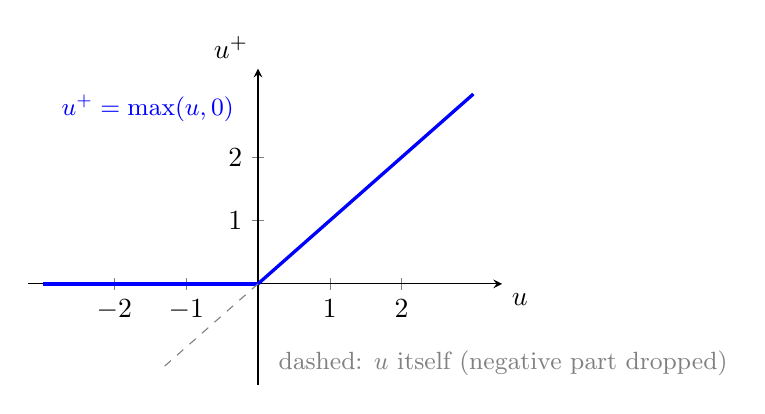
\begin{tikzpicture}
	\begin{axis}[
		axis lines=middle, xmin=-3.2, xmax=3.4, ymin=-1.6, ymax=3.4,
		xtick={-2,-1,1,2}, ytick={1,2},
		xlabel={$u$}, ylabel={$u^+$}, xlabel style={below right}, ylabel style={above left},
		width=7.6cm, height=5.6cm, clip=false
		]
		\addplot[blue, very thick, samples=2, domain=-3:0] {0};
		\addplot[blue, very thick, samples=2, domain=0:3] {x};
		\addplot[gray, dashed, samples=2, domain=-1.3:0] {x};
		\node[blue, anchor=south east, font=\small] at (axis cs:-0.2,2.4) {$u^+=\max(u,0)$};
		\node[gray, anchor=west, font=\small] at (axis cs:0.15,-1.25) {dashed: $u$ itself (negative part dropped)};
	\end{axis}
	\end{tikzpicture}
\end{document}
